En este capítulo se expondrán los conceptos más importantes para nuestra propuesta. Hablaremos sobre conceptos de la computación de alto rendimiento que se utilizarán para poder evaluar el trabajo realizado de forma cuantitativa. Seguidamente se expondrán las simulaciones sísmicas más utilizadas y se darán criterios para escoger aquella con la que se trabajará durante el proyecto. Finalmente, se hablará sobre el análisis y simulación in-situ, se mostrará los ejes en los que se caracterizan las bibliotecas y se expondrán las principales.
\section{Computación de alto rendimiento}
La computación de alto rendimiento, o HPC por sus siglas en inglés, hace uso de conocimientos de distintas áreas de la ciencia y la computación para hacer uso de computadoras y clústers de computadoras de forma eficiente. Se ha dicho que informalmente el HPC es un área científica y técnica que estudia las supercomputadoras~\cite{Nielsen2016}. Este trabajo es parte busca aplicar el HPC a un problema científico por lo que es necesario tener claro algunos conceptos.
\subsection{Rendimiento}
Definimos rendimiento (o performance en inglés) como el recíproco del tiempo de ejecución de un programa~\cite{Hennessy2017-ml}. Esto se puede expresar matemáticamente en la~\cref{eq:performance}.
\begin{equation}
  p_{a} = \frac{1}{t_a}
  \label{eq:performance}
\end{equation}
Cuando comparamos dos implementaciones de un programa podemos hacerlo con sus rendimientos o sus tiempos de ejecución. Podemos expresar que un programa $a$ es $n$ veces más rápido que un programa $b$ con la~\cref{eq:comparison}.

\begin{equation}
  n = \frac{p_a}{p_b} = \frac{t_b}{t_a}
  \label{eq:comparison}
\end{equation}

\subsection{Speedup}
El speedup es la razón entre el rendimiento de un programa que ha sido mejorado y el mismo programa antes de la mejoría~\cite{Hennessy2017-ml}. Esta mejoría puede ser un cambio en el programa en sí, o en los recursos computacionales que tiene disponibles.
En HPC nos interesa medir el speedup de un programa a distintas cantidades de nodos en una supercomputadora específica. El speedup $s$ de un programa utilizando $n$ nodos de computación está dado por la~\cref{eq:speedup}
\begin{equation}
  s_n = \frac{t_1}{t_n} = \frac{p_n}{p_1}
  \label{eq:speedup}
\end{equation}
\subsection{Ley de Amdahl}
La ley de Amdahl se refiere a la observación hecha por Gene Amdahl de que todos los programas están conformados por una fracción que se ejecuta de forma serial ($r_s$) y otra que se puede ejecutar de forma paralela ($r_p$)~\cite{amdahl1967}. A esta fracción serial le llamamos overhead. El tiempo de un programa que se ejecuta con un sólo procesador sería entonces:
$$t_1 = t_s + t_p = 1$$
Donde $t_p$ se refiere al tiempo que le programa dura en la fracción que se puede paralelizar, $t_s$ el tiempo que dura en la fracción serial y lo definimos como 1 para facilitar los cálculos posteriores.
Si ejecutamos el programa con $N$ procesadores el tiempo sería ahora:
$$t_N = t_s + \frac{t_p}{N}$$
Utilizando la~\cref{eq:speedup} el speedup sería:
\begin{equation}
  s_N = \frac{1}{t_s + \frac{t_p}{N}}
  \label{eq:amdahl}
\end{equation}
La~\cref{eq:amdahl} es lo que conocemos como la ley de Amdahl. Tomando el límite de esta ecuación observamos lo siguiente:
$$\lim_{N\to\infty} \frac{1}{t_s + \frac{t_p}{N}} = \frac{1}{t_s}$$
El speedup está acotado por el overhead del programa.
\subsection{Ley de Gustafson-Barsis}
Gustafson y Barsis observaron que la ley de Amdahl tiene una suposición implícita, el tamaño del problema de entrada del programa se mantiene fijo con respecto a la cantidad de recursos computacionales disponibles~\cite{Gustafson1988}. De acuerdo a su experiencia trabajando en el Laboratorio Nacional Sandia en los Estados Unidos esto no es una suposición realista, el tamaño de los problemas que los investigadores resuelven está relacionado con la cantidad de recursos que tienen disponibles. Adicionalmente los autores notaron que el overhead del programa era aproximadamente independiente del tamaño del problema. Los autores entonces proponen que el tiempo de ejecución de un programa paralelo con $N$ nodos está dado por:
$$t_N = t_s + t_{p_n} = 1$$
Aquí de nuevo $t_s$ es el tiempo que el programa invierte en la fracción secuencial, pero $t_{p_n}$ se refiere al tiempo que el programa pasa en la fracción paralela del programa con una carga de trabajo distribuida. Definimos la ecuación como 1 para facilitar los cálculos.
De aquí tenemos que el tiempo de ejecución del mismo programa con la misma carga de trabajo de forma serial sería:
$$t_1 = t_s + t_{p_n}\times N$$
Por lo que el speedup es:
\begin{equation}
  s = \frac{t_1}{t_N} = t_s + t_{p_n}\times N
  \label{eq:gustafson}
\end{equation}

La~\cref{eq:gustafson} se conoce como la ley de Gustafson-Barsis. Es importante recalcar que la ley de Amdahl y la ley de Gustafson-Barsis miden el speedup de dos situaciones distintas, por una parte la ley de Amdahl supone que el programa tiene una carga de trabajo constante y simplemente se le están dando más recursos de ejecución, mientras que la ley de Gustafson-Baris supone que la carga de trabajo crece con la cantidad de recursos disponibles.
\subsection{Escalabilidad}
La escalabilidad se refiere a la forma en que cambia la eficiencia de un programa al cambiar el tamaño del problema o los recursos computacionales disponibles~\cite{Pacheco2011-sb}.
\subsubsection{Escalamiento fuerte}
El escalamiento fuerte se refiere al escalamiento de un programa cuando el tamaño del problema se mantiene constante pero se cambia la cantidad de recursos computacionales~\cite{Pacheco2011-sb}. La ley de Amdahl (\cref{eq:amdahl}) nos dice que mantener el escalamiento fuerte es difícil de mantener~\cite{Mattson2019-vv}.
\subsubsection{Escalamiento débil}
El escalamiento débil es el estudio del escalamiento de un programa cuando se hace que el tamaño del problema cambie de forma proporcional a la cantidad de recursos computacionales~\cite{Pacheco2011-sb}. Si el overhead de manejar los recursos paralelos se mantiene relativamente constante, la ley de Gustafson-Barsis (\cref{eq:gustafson}) predice que el tiempo de ejecución será constante, por lo que este tipo de escalamiento sirve para determinar el overhead de los programas~\cite{Mattson2019-vv}.
\section{Simulaciones sísmicas}
En esta sección se enumerarán las simulaciones sísmicas de código abierto más importantes para nuestro proyecto y se argumentará la escogencia de una de estas. La inclusión de estas simulaciones en esta lista se basa en que son parte del proyecto ChEESE de la Unión Europea que consiste en centros de excelencia para el desarrollo de software relacionado a ciencias de la tierra sólida~\cite{Folch2023}. Adicionalmente se incluye el software AWP-ODC que ha sido utilizado en el pasado para demostrar capacidades de bibliotecas in-situ~\cite{mu_-situ_2019}. Nuestros criterios para escoger una simulación son los siguientes:
\begin{itemize}
    \item Familiaridad con el lenguaje de programación.
    \item Que la biblioteca esté bajo desarrollo activo.
    \item Que el desarrollo de la simulación no esté condicionada a proyectos.
\end{itemize}

Mostramos un resumen de las bibliotecas en el~\cref{tab:seismic_simulations}. Tomando en cuenta estos criterios decidimos escoger la biblioteca SeisSol para el desarrollo de este proyecto.

% Ecuaciones de onda
% Ondas P
% Ondas S
\subsection{SPECFEM}
SPECFEM~\cite{Peter_Forward_and_adjoint_2011} es una familia de simulaciones sísmicas que hacen uso del método finito estocástico espectral para realizar simulaciones de propagación de ondas sísmicas a distintas escalas. Está mayormente desarrollado en FORTRAN, con una versión en C++.
Las simulaciones que forman parte de esta familia son:
\begin{itemize}
  \item \textbf{SPECFEM2D}: Permite realizar simulaciones de propagación de ondas acústicas y elásticas en 2 dimensiones.
  \item \textbf{SPECFEM3D\_Cartesian}: Permite realizar simulaciones de propagación de ondas sísmicas en escalas locales o regionales y realizar la tomología correspondiente.
  \item \textbf{SPECFEM3D\_GLOBE}: Similar al punto anterior, este software permite la simulación de ondas sísmicas, pero en este caso a escala global o continental. La diferencia entre uno y otro está en el mallado que se puede utilizar, así como las optimizaciones que se realizan.
  \item \textbf{SPECFEM++}: Esta es una versión de los softwares anteriores desarrollada en C++. Aún se encuentra muy atrás con respecto a las otras versiones.\end{itemize}

Debido a que la versión en C++ aún no está lista para producción y que no se maneja el lenguaje FORTRAN decidimos excluir esta simulación.

\subsection{ExaHyPE 2}
Esta simulación también se basa en el método de Galerkin discontinuo~\cite{Reinarz2020}. Permite realizar un mallado adaptativo. Se puede utilizar para modelar todo tipo de ecuaciones diferenciales parciales hiperbólicas, no únicamente aquellas relacionadas a la sismología. Se realizaron pruebas de escalamiento, hasta llegar a los 28 nodos con un total de 784 núcleos. El software está escrito en C++ con porciones en FORTRAN y Python y actualmente su desarrollo está circumscrito a la biblioteca de mallado cartesiano, Peano. Debido a esta forma de desarrollar la simulación de forma acoplada a la biblioteca Peano se decidió no utilizar esta biblioteca en el proyecto.

\subsection{AWP-ODC}
AWP-ODC hace uso de un método de diferencias finitas~\cite{Cui2010}. Permite realizar simulaciones de propagación de ondas sísmicas, así como el modelado de rupturas dinámicas en fallas verticales. Este software intenta resolver el problema de la E/S utilizando MPI-IO para realizar entrada y salida paralela. Luego de revisar el repositorio de código de esta simulación se determinó que la misma no está bajo desarrollo activo~\cite{githubGitHubHPGeoCawpodcos}.

\subsection{SeisSol}
SeisSol~\cite{Kser2010} permite la simulación de la propagación de ondas sísmicas y de rupturas dinámicas utilizando un método de Galerkin discontinuo. El método de mallado que utiliza esta simulación le permite adaptarse a materiales altamente híbridos. En el artículo que presenta este software, se demuestra que el software logra escalar satisfactoriamente hasta los 1024 núcleos, con una eficiencia del 76\%. Se utilizó para realizar la simulación de ruptura dinámica más larga y grande en el 2017 con una simulación del terremoto del océano Índico del 2004~\cite{Uphoff2017}. El software está implementado en C++. Debido a que esta simulación cumple con nuestros criterios se decidió que se utilizaría para el desarrollo de este proyecto.

\section{Análisis in-situ}
En este trabajo, se utilizarán los términos ``análisis in-situ'' y ``visualización in-situ'' para referirse al análisis y simulación que se realiza de forma simultánea a la ejecución de la simulación que genera los datos, independientemente de si este análisis se realiza en el mismo hardware que la simulación o si este se transporta hacia un hardware dedicado a realizar estas tareas~\cite{childs_terminology_2020}.

\begin{table}
    \centering
    \begin{tabular}{|p{0.17\linewidth}|p{0.14\linewidth}|p{0.20\linewidth}|p{0.17\linewidth}|}
    \hline
         Nombre & Lenguaje & Desarrollo activo & Autónomo \\
         \hline
         SPECFEM3D & FORTRAN & Sí & Sí \\ 
         \hline
         SeisSol & C++ & Sí & Sí \\
         \hline
         ExaHyPE 2 & C++ & Sí & No \\
         \hline
         AWP-ODC & C & No & Sí \\
         \hline
         
    \end{tabular}
    \caption{Resumen de simulaciones sísmicas}
    \label{tab:seismic_simulations}
\end{table}

\begin{figure}
  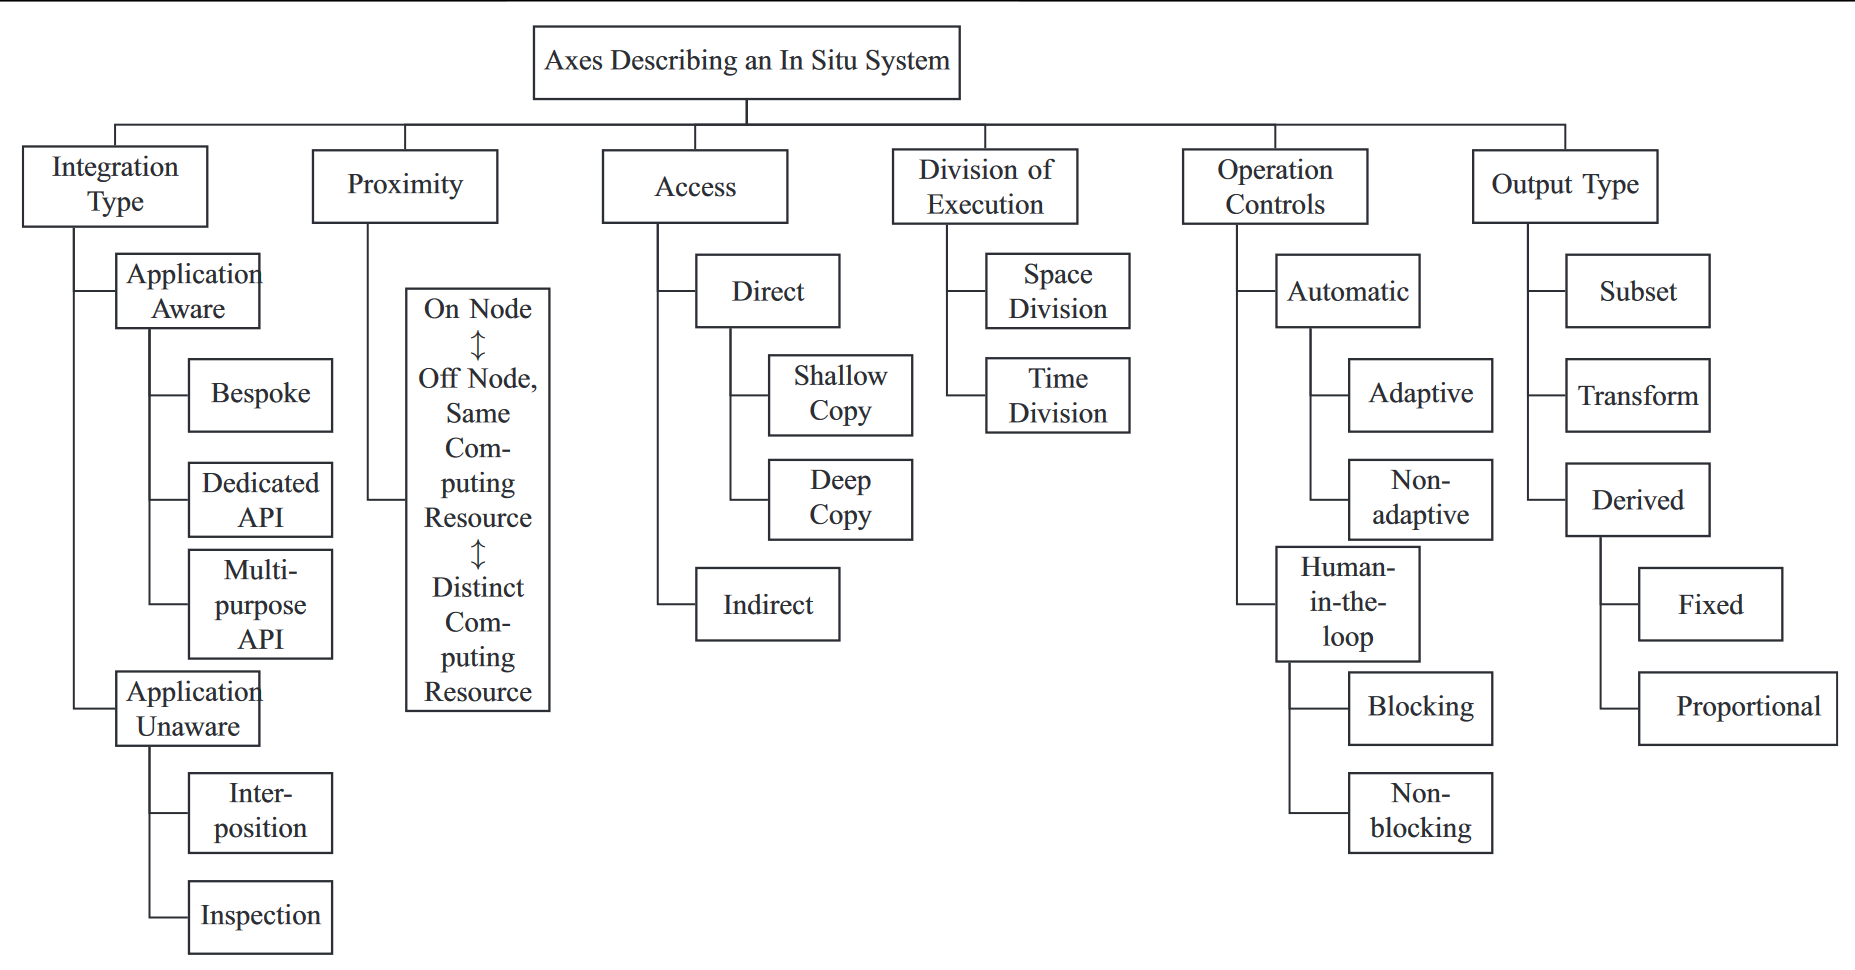
\includegraphics[width=\textwidth]{insitusystems}
  \caption{Características utilizadas para clasificar las bibliotecas in-situ.}
  \label{fig:insitusystems}
  
\end{figure}
\subsection{Caracterización de bibliotecas de análisis in-situ}
En la \cref{fig:insitusystems}, tomada de~\cite{childs_terminology_2020} se pueden observar los seis ejes con los que es posible realizar una caracterización las bibliotecas de visualización y análisis in-situ.
\begin{enumerate}
  \item Tipo de integración con la simulación.
  \item Proximidad del código de análisis y visualización de la simulación.
  \item El acceso de las bibliotecas a los punteros de los datos.
  \item La forma en la que se divide el tiempo o espacio de ejecución.
  \item Controles que se tienen sobre la simulación mientras se ejecuta.
  \item Tipo de salida.
\end{enumerate}
\subsection{Bibliotecas de análisis y visualización in-situ}
\subsubsection{ADIOS2}
Esta biblioteca~\cite{Godoy2020} le permite al usuario realizar transferencias de datos entre unidades de ejecución de forma transparente, ya sea que es entre dos nodos de una supercomputadora conectadas por alguna red de interconexión como Infiniband, entre computadoras regulares conectadas por internet e incluso entre computadoras regulares y supercomputadoras.
Tiene tres APIs diseñadas con distintos niveles de abstracción.
\begin{itemize}
  \item El API de alto nivel está pensado para flujos de trabajo de análisis de datos. Tiene bindings para C++, Python y Matlab.
  \item El API de bajo nivel está diseñado para ser integrado en simulaciones de HPC. Está basado en MPI para reducir los costos de comunicación de red.
  \item El API privado permite desarrollar ADIOS con prácticas modernas de ingeniería de software.
\end{itemize}

Tomando en cuenta los ejes mencionados anteriormente ADIOS2 se clasifica de la siguiente manera~\cite{childs_terminology_2020}: 
\begin{itemize}
    \item API multipropósito.
    \item Puede ser utilizada tanto en el mismo nodo, en otro nodo dentro del mismo recurso computacional y de forma completamente remota.
    \item Acceso directo a los datos mediante copias superficiales. También es posible realizar accesos indirectos.
    \item El análisis de datos se puede realizar dividiendo tanto el tiempo como el espacio de ejecución.
    \item Permite la implementación de cualquier tipo de interacción con la simulación.
    \item Igualmente, permite que la salida de la simulación se ajuste a lo que los desarrolladores de la simulación encuentren necesario.
\end{itemize}

\subsubsection{Catalyst}
Es una herramienta desarrollada por Kitware como un acompañante al software de visualización científica Paraview, aunque es posible utlizarla de manera autónoma. Permite instrumentar el código de la simulación mediante el estándard de descripción de datos científicos, Conduit~\cite{Ayachit2021}.

Catalyst se clasifica de la siguiente manera, de acuerdo a~\cite{childs_terminology_2020}:
\begin{itemize}
    \item API dedicado a la visualización.
    \item Procesamiento en el mismo nodo, aunque es posible hacer uso de ADIOS2 para realizar también procesamiento en otro nodo.
    \item Tiene acceso directo a los datos mediante copias superficiales de estos.
    \item Hace una separación entre la simulación y la visualización en el tiempo.
    \item De forma nativa no permite realizar el manejo automático del análisis dependiendo de las condiciones que estén sucediendo en la simulación.
    \item Permite tener una salida de datos derivados de la simulación original.
\end{itemize}

\subsubsection{Ascent}
Es una biblioteca de peso ligero diseña desde un principio para que ejecute directamente en el mismo nodo que la simulación \cite{Larsen2022}. Es bastante flexible y puede interactuar con ADIOS2 y Catalyst. Permite realizar tanto analisis como visualización in-situ y tiene un sistema de disparadores que permite realizar un control automático de la simulación mientras esta se ejecuta.

Bajo la taxonomía de~\cite{childs_terminology_2020}, Ascent se clasifica de la siguiente manera:
\begin{itemize}
    \item API multipropósito.
    \item Procesamiento en el mismo nodo.
    \item Acceso directo a los datos mediante copias superficiales así como con copias profundas de datos.
    \item Divide la ejecución de los programas en el tiempo.
    \item Permite un manejo automático pero no adaptativo de la simulación gracias a su sistema de disparadores.
    \item Permite cualquier tipo de salida que el programador encuentre necesaria.
\end{itemize}